% !TEX root = DesignDocument.tex


\chapter{Overview and Concept of Operations}

%The overview should take the form of an executive summary.  Give the reader a feel 
%for the purpose of the document, what is contained in the document, and an idea 
%of the purpose for the system or product. 

\section{Bowtaps and Its Team}

Bowtaps is a start up company from Rapid City, SD that began working together at the SDSM\&T campus. Our goal is to create easy to use software applications that help ease the everyday life of the user. Their software aims to be both well-constructed and maintainable, and their products are made with sustainability in mind. Bowtaps currently consists of the members Charles Bonn, Johnathan Ackerman, Daniel Andrus, Evan Hammer, and Joesph Mowry. Their roles and experience are further detailed in section C of this document.

\section{Crowd Control}
Crowd Control is our flagship product designed and created by Bowtaps. Its goal is to combine GPS tracking, group messaging and group management features into one easy to use application. A primary focus of this product is to be maintainable and modular, so that if better solutions arise, those can be implemented with minimal refactoring.

User information is perhaps our greatest focus in Crowd Control's design; careful measures were taken to assure that sensitive user information is kept safely, vulnerabilities are removed, and risks are mitigated. Before Crowd Control is released to the public, we will implement an encryption scheme called AES-256. Bowtaps also uses third-party services such as Parse and Sinch that guarantee safety in storage and transmission of data through their access points.

Crowd Control, in addition to being written in a maintainable, well-designed manner, is aimed to be a sustainable commercial product. Bowtaps is using what they have gathered from various business accelerators and entrepreneurship-focused learning material to apply those concepts to the real-life startup company, Bowtaps, LLC. Bowtaps uses their recently acquired business skills to market Crowd Control, project associated finances, and seek investors for expansion.

\subsection{Purpose of the System}
Crowd Control is a mobile application designed to ease the experience of going out though the implementation of integrated group messaging, GPS tracking and group management features. Along with the features to manage your group at the event Crowd Control also gives suggestions of local events, restaurants and attraction. This allows the group to continue even when the next item on the agenda is a mystery. 

Even though Crowd Control is initially designed for the event-goer scene, it's uses can be expanded to fit more purposes. Crowd Control can be used to help manage any kind of group at an event such as church groups, tour groups, or school field trips.

\section{Business Need}
\begin{comment}
Use this section to define what business need exist and how this software will 
meet and/or exceed that business need.   (still fill out)
\end{comment}

Currently, there is no product on the market that encompasses all the features of group management, in-app messaging, and GPS tracking in one easy-to-use package. For example, Facebook is a popular option for group messaging and event creation, but it doesn't allow users to track each other for a duration of time. Crowd Control allows for both group messaging and event creation, as well as GPS tracking and better group management, specifically tailored to those at an event. Facebook's limited group management features are specifically designed for planning an event ahead-of-time, not necessarily managing during an event.

Crowd Control not only addresses the needs of those seeking group management/communication during events, but also helps serve as a platform for businesses to advertise themselves to users in the form of events and promotions. Those events are available in the form of nearby events that users can choose to set as their destination upon creating a group. This is a mutually beneficial feature for the users and for the businesses themselves.

\section{Deliverables}
\begin{comment}
Provide a complete description of the client requested deliverables.   This section should be the section your software contract references.   ( still fill out)
\end{comment}
The deliverables for this two-semester senior design project are the following items:
	\begin{itemize}
	  \item Crowd Control mobile application
	  \item Associated JavaDoc documentation
	  \item Senior Design document - some included items include:
	  	\begin{itemize}
		  \item General documentation
		  \item User manual and various code documentation
		  \item Business plan for Bowtaps, LLC
		  \item Sprint reports
		\end{itemize}
	  \item Design fair presentation
	\end{itemize}


\section{System Description}
Behind the UI, Crowd Control is written using an MVC architecture. IOS is written natively in Swift under the IDE XCode. On the Android side, the code is written in Native Mobile Java under Android Studio.

The code for Android uses XML files for storing layout-related code, which act as the view in the MVC pattern. Each activity acts as a controller. Each one of the models has an interface, which is how the controllers get access to the functions and data provided by the model. Each interface is set up in such a way that it uses OOP inheritance to generalize the models, thus abstracting our third party software. This contract allows us to write our code in such a way that, if ever needed, we could change the underlying implementation of certain modules with minimal refactoring.\\\\
%Remove explicit newlines after iOS section is taken care of.
The iOS platform follows a very similar MVC design pattern, too.\\
(TODO: iOS details needed.)

\subsection{Integrated Group Messaging}
Integrated group messaging is an important feature of Crowd Control. It allows for communication across different platforms, different phone brands, and different carriers. This allows for seamless communication between users without the issues associated with SMS such as messages not using the same format, messages not going to all recipients, and messages with users in the group that you do not want to have your personal information.

Bowtaps integrates a third-party called Sinch as our message-handling service. Sinch handles the encryption of messages to ensure security of user data. Sinch uses app to app messaging, so that any device running Crowd Control can send a message to other group members, independent of platform or carrier. However, since our app is currently only fully implemented on Android, messages can only be passed between Android users.

\subsection{GPS Location Services}
Crowd Control utilizes GPS functionality to track users that belong to groups through the Google Play services location application program interfaces (APIs). This allows users to find fellow group members by retrieving their current or last known location. This is useful to help locate members of the group that maybe lost or unable to be located, perhaps towards the end of an event, or when group members want to meet up again.

Because GPS functionality can draw heavily from a device's power supply, users are able to opt out of a GPS retrieval on their device. If a user does not want to have their location known to the group, or simply has a low battery level, their GPS retrieval can be shut off. Alternatively, when the user's battery is low, it will allow for the GPS check-in interval to be extended or turned off completely to save battery life.

\subsection{Group Management Features}
Perhaps the most important feature set, are those pertaining to group management. The party leader sets the initial information for a group for the other members to view and interact with. The party leader can edit certain information about the group, and even kick certain members if needed. A group management menu allows for a group agenda to be posted, updating members when the agenda changes. Pairing with the GPS features, Crowd Control also allows for the group leader to set way-points for the group.  

\subsection{Suggestions}
Sponsorship by local businesses take the form of an unobtrusive advertisement called a ``suggestion''. Suggestions are both a plus for the user and serve as our way of making revenue. Although these are not traditional ads, they alert the user to local points of interest such as restaurants, bars, amusement parks, concerts, and many more. With our suggestion interface, users can browse events for their group to attend while local businesses gain exposure, and we gain revenue.

\section{System Overview and Diagram}
The basic overview of Crowd Control can be seen in the diagram below. See Figure~\ref{ModuleFlowDiagram}. Crowd Control will be using a model-view-controller design structure. With the model view controller design method we are able to abstract the user interface from the control structures that will communicate with the third party services such as Parse, Google play services, or Sinch. The model of each respective operating system ( Android or iOS ) will be able to communicate with the respective mapping feature ( Google Play Services or Apple Map Features ). While both models will be able to communicate with Parse, our back end server. Though Parse, using their features, will be able to connect user profiles to their Facebook and twitter accounts for faster log in.

\begin{figure}[tbh]
\begin{center}
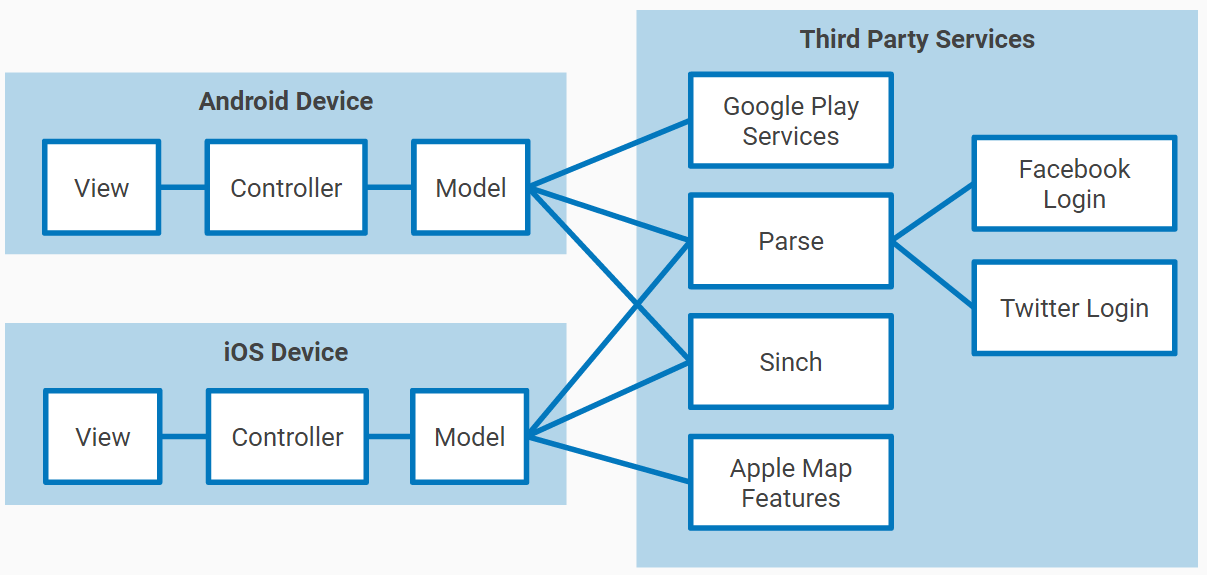
\includegraphics[width=0.75\textwidth]{Additional/designpictures/ModuleFlowDiagram2.png}
\end{center}
\caption{Basic System Flow Diagram \label{ModuleFlowDiagram}}
\end{figure}

\section{Technologies Overview}
Crowd Control accesses various different external technology entities. Some technologies used in the creation of Crowd Control are Google Play Services, Apple Map Features, Parse, Sinch, and Android Studio.

\subsection{Google Play Services}
	\subsubsection{Description}
	Google Play Services contains a number of APIs that allows Crowd Control to access Google-powered features. One such feature is Google Maps, which allows the app to access mapping capabilities managed by Google. Using their API, users can place pins and find their friends on a map that is smoothly integrated into Crowd Control, without Bowtaps having to maintain the map functionality.
\newline
REFERENCE LINK:  \url{https://developers.google.com/android/guides/setup}
	\subsubsection{Usage}
	Google Play Services will be used on the Android device as the default map. Google Play Services provides a more native feel to Android users when interacting with mapping features. This allows for a more consistent user experience when it comes to using Crowd Control. At a set interval which can be changed, the map is updated with the user's current location, as well as all other users in the group. From the map, data is securely stored and transmitted safely to other group members.

\subsection{Apple Map Features}
	\subsubsection{Description}
	Apple Map Features is the native iOS API for mapping features. With this it allows for commiseration between a map and your gps location along with other mapping features.
\newline
REFERENCE LINK: \url{https://developer.apple.com/maps/}
	\subsubsection{Usage}
	Apple Map Features will be used on the iOS device as default. We chose to go with Apple Map Features to give iOS users a more native, less intrusive feel. This will be used for displaying your location, displaying other users from your group, and displaying local event suggestions on the map.

\subsection{Parse}
	\subsubsection{Description}
	Parse is a third-party service that serves as a secure no-SQL datastore. The service is free under a certain number amount of data transacted to and from Parse. The Parse API allows Crowd Control to access various methods to store and fetch data pertaining to the datastore. It should be noted that Parse will cease server hosting in January of 2017. Parse has provided tools to migrate existing applications to use another database solution such as MongoDB.
\newline
REFERENCE LINK: \url{http://parse.com/}
	\subsubsection{Usage}
	Crowd Control currently saves all group and user information on Parse servers. This data is to be considered sensitive and is treated with the utmost consideration for security and protecting that data. Some data is also cached to the local device, to both reduce data transmission to and from the server, as well as increasing the speed of the user's overall performance. Some of the cached data includes any previous existing user data and group data, so that if the user closes the app, they should not need to re-enter their login information. 
	
\subsection{Sinch}
	\subsubsection{Description}
	Sinch is a third party device-to-device communication API. Bowtaps selected it for its built-in encryption, and ready-to-use messaging platform. The Sinch API provides message-passing functionality various message broadcasting methods. This platform requires either a Wi-Fi connection, or cellular data service. 
\newline
REFERENCE LINK: \url{https://www.sinch.com/}
	
	\subsubsection{Usage}
	Sinch ables Crowd Control to handle the sending and receiving of messages between group members. Through use of the Sinch help manuals, Bowtaps has constructed a fragment to control a user interface that fetches messages sent by users. We have also modified the basic one-to-one message sending implementation to broadcast the message to the entire group.



